\chapter{Smart Grid}

\section{Instalação e Coleta}

O conceito de redes inteligentes está ligado ao uso de elementos digitais e de comunicações nas redes que transportam a energia. Esses elementos possibilitam o envio de diversos dados e informação para os centros de controle, onde eles são tratados, auxiliando na operação e controle do sistema como um todo. Para isso deve-se colocar em pratica algumas transformações, como a modernização da infraestrutura, instalação de softwares e capacidade de processamento desses dados. Com isso para a instalação das Redes Inteligentes, algumas etapas devem estar associadas como a medição eletrônica, a comunicação, o sensoriamento e a computação tais sistemas estão correlacionados a um medidor inteligente e a um sistema de comunicação.

\subsection{Medição Eletrônica}

	O controle de perdas, planejamento e operação da rede estão diretamente ligados a essa tecnologia sendo assim tal medição está envolvida desde a geração até o uso final. Com a introdução desse tipo medidor, o consumidor terá mais condições de gerenciar seu uso de energia. Vários aplicativos já estão em desenvolvimento para proporcionar o acesso aos dados de medição, auxiliando na tomada de decisão. Dados como consumo em tempo real, equipamentos que mais consomem energia, valor a pagar até o momento, projeção de fatura no final do ciclo são alguns exemplos de interação entre usuário e medidor. Outros serviços ainda podem ser agregados, como por exemplo, o controle de cargas pelo usuário. Antes mesmo de chegar à sua casa, o consumidor poderá programar qualquer equipamento conectado à rede elétrica.


\begin{figure}[H]
 \begin{center}
	
\includegraphics[keepaspectratio,scale=1.5,angle=0]{figuras/medidor_eletronico.eps}
	\caption{Medidor eletrônico}
 \end{center}
\end{figure}

\subsection{Comunicação}

	Uma das funcionalidades mais importantes dos medidores inteligentes é a capacidade de se comunicar com outros equipamentos instalados na rede ou mesmo dentro das unidades consumidoras. Para que o conceito de redes inteligentes seja totalmente viabilizado, é necessário que essa comunicação seja feita em duas direções – da central para o usuário e vice-versa. Funções como a suspensão e religação de fornecimento remotas, envio de informação sobre consumo em tempo real dependem dessa comunicação bidirecional.

	Quando os diversos sistemas e seus componentes possuem a habilidade de operarem em conjunto, alcançamos o conceito de interoperabilidade (capacidade de diversos sistemas trabalharem em conjunto). Permitindo a integração, o funcionamento cooperado e a comunicação bidirecional entre os vários elementos interconectados do sistema elétrico. Para que seja efetiva, deverá ser estruturada uma padronização de interfaces, protocolos e outros elementos de interconexão, utilizando softwares e assim eles possam trocar informações entre si.

\subsection{Sensoriamento}

	A instalação de sensores ao longo de todo o sistema de distribuição de energia elétrica é outro passo para que a rede se torne realmente inteligente. A auto recuperação, uma das responsáveis pela diminuição das faltas de energia, é beneficiada com o sensoriamento da rede. Os sensores são responsáveis por enviar as informações para a central de controle que ao receber dados toma-se uma decisão. A automatização será uma realidade e o religamento de áreas afetadas poderá ser feito mais rapidamente, eliminando o desconforto dos usuários e aumentando a receita.

	Sensores são embutidos com chips que detectam informações sobre a operação e desempenho da rede, tais como tensão e corrente. Então, analisam essas informações para determinar o que é significativo - por exemplo, está com tensão muito alta ou muito baixa. Quando se detecta informações significativas ocorre a comunicação dos dados para um sistema de software armazenando no mesmo\cite{2015Salema}.

\subsection{Computação}

	O processamento dos dados recebidos por todos os equipamentos da rede irá aumentar substancialmente, por isso, torna-se necessário que os centros de controle que sejam capazes de transformá-los em informações úteis para os usuários. Muitos dados disponíveis podem tornar confusa a leitura e a decisão pode ser equivocada e piorar as condições da rede sendo necessário um filtro desses dados.

	É esperado grande volume de dados causado por grande número de fontes de tráfego ou por alta intensidade na demanda de dados. Em sistemas SCADA tipicamente há um fluxo intenso de limitadas fontes de tráfego fornecendo dados para uma unidade concentradora, ao qual incluem dispositivos eletrônicos inteligentes.

\subsection{Medidor Inteligente}

	O medidor inteligente irá interligar a casa ao restante da rede. O primeiro ponto de recepção desses dados será o concentrador. Ele pode receber informações de um grande número de medidores e, então, enviá-las para pontos de retransmissão como torres, e destas, para subestações ou outros pontos, para depois serem transmitidos para os centros de controle da distribuição. Dentro das residências também teremos novidades. Ao se criar uma rede doméstica centrada no medidor, vários serviços poderão ser oferecidos e haverá um novo relacionamento entre cliente e concessionária, bem como uma nova relação entre o consumidor e seu uso da energia.

	É um dos componentes principais de todo o sistema. Ele é o responsável pela maioria das funcionalidades de uma rede inteligente. Capaz de processar dados e enviar comandos para vários outros equipamentos, permitindo a integração de toda a cadeia de fornecimento. Além de medir o consumo em intervalos programados, o medidor inteligente se utiliza de uma combinação de tecnologias, como sensores de tempo real, notificação de falta de suprimento e monitoramento da qualidade da energia.

	Na casa sustentável serão utilizadas fontes de energia limpa. As fontes de energia limpa, como eólica e solar, são também intermitentes. Por isso, sua integração à rede se torna complexa. Nesse ponto, as tecnologias que podem ser agregadas à rede são de fundamental importância para a introdução desse tipo de geração. E estamos falando da microgeração, que poderão atender a casa. Essa integração deverá ser completa, possibilitado a participação de todos os agentes do setor.

	Geralmente, tem-se usado a tecnologia ZibBee. Todo equipamento com esse tipo de conexão poderá se comunicar com o medidor, transmitindo e recebendo informações e comandos. Se o consumidor permitir, a concessionária terá a capacidade de controlar a carga dentro de cada residência, como, por exemplo, regular a temperatura de aparelhos através dos termostatos inteligentes, ou, até mesmo, ligar e desligar cargas. Dessa forma, as concessionárias poderão limitar a demanda e evitar sobrecargas nas redes. Outra forma de limitar os picos de demanda é a tarifação diferenciada por postos horários. Como o medidor pode registrar o consumo em diferentes períodos ao longo do dia, poderão ser aplicadas maiores tarifas em horários de maior concentração de demanda, evitando que muitos consumidores usem a energia ao mesmo tempo, aliviando o sistema\cite{2015Zimmermann}.

	Existem três tipos diferentes de dispositivos ZigBee: ZigBee coordenador (ZC): O dispositivo mais completo, o coordenador faz a raiz da árvore da rede e pode superar a outras redes. Há exatamente um coordenador ZigBee em cada rede, ele é capaz de armazenar informações sobre a rede, inclusive atuando como o Centro de Fidedignidade e repositório de chaves de segurança. ZigBee Router (ZR): Assim como executar uma função do aplicativo, um roteador pode funcionar como um roteador intermediário, transmissão de dados de outros dispositivos. ZigBee dispositivo final (ZED): Contém a funcionalidade apenas o suficiente para falar com o nó pai (ou coordenador ou um roteador), ele não pode transmitir dados de outros dispositivos. Esta relação permite que o nó a ser adormecido uma quantidade significativa do tempo dando assim a vida da bateria longa. Um ZED requer a menor quantidade de memória, e, portanto, pode ser menos caro de fabricar do que um ZR ou ZC.

\subsection{Sistemas de Comunicação}

	Inúmeras tecnologias estão disponíveis no mercado para a transmissão de dados entre a unidade consumidora e os centros de operação das concessionárias. A escolha deverá se basear na necessidade de confiabilidade, segurança e disponibilidade de cada serviço oferecido. Podemos observar quatro camadas na área de telecomunicações: HAN –Home Area Network –, LAN – Local Area Network –, RAN – Regional Area Network – e WAN – Wide Area Network.

\begin{figure}[H]
 \begin{center}
	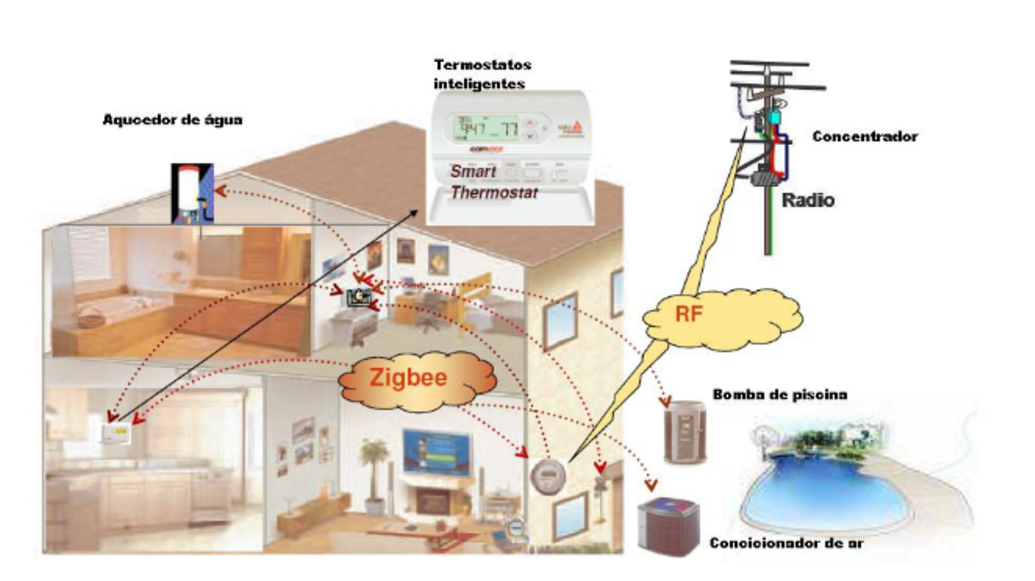
\includegraphics[keepaspectratio]{figuras/zigbee.eps}
	\caption{Zigbee}
 \end{center}
\end{figure}

	Na casa sustentável iremos utilizar A HAN abrange a residência e não deverá apresentar grandes entraves na questão da comunicação de dados. Podem ser usadas as tecnologias Wireless, como ZibBee, ou mesmo a PLC. É necessário definir soluções que garantam a integridade de dados transmitidos de forma a evitar possíveis fraudes, ou ataques aos sistemas de informação, como por exemplo, medição eletrônica. Também é necessário definir autenticidade de entidades que transmitem e das que recebem dados. Há necessidade de proteções contra violação de informação em medidores eletrônicos, por exemplo, ao atualizar firmware de dispositivos\cite{2013Atmel}\cite{2013RiveraEspositoTeixeira}.

	Um sistema de comunicação é a componente chave para a infraestrutura Smart Grid, e o PLC é uma das principais tecnologias de comunicação disponíveis para este fim. A tecnologia PLC é uma técnica que utiliza a rede elétrica para transmitir, a altas taxas de transmissão, sinais de dados entre dispositivos. Em uma rede PLC, medidores inteligentes podem estar ligados a um concentrador de dados por meio da rede elétrica e transferir as informações para uma central de dados. A infraestrutura da rede elétrica existente diminui os custos de instalação relativos a um sistema de comunicações, sendo bastante adequada em áreas urbanas para diversas aplicações.

\begin{figure}[H]
 \begin{center}
	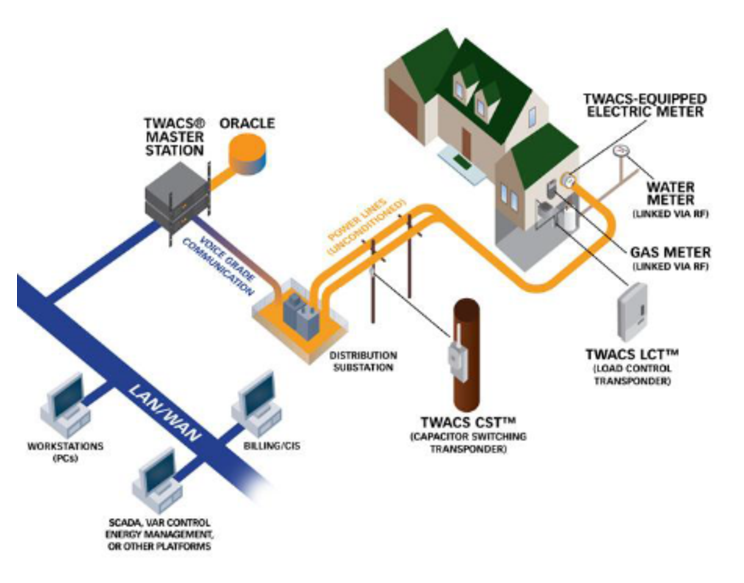
\includegraphics[keepaspectratio]{figuras/exemplo_plc.eps}
	\caption{Exemplo de aplicação do PLC}
 \end{center}
\end{figure}

	Neste contexto, é proposto o desenvolvimento de um circuito PLC para operar na faixa de banda estreita. Neste trabalho, foi selecionada a frequência de operação de 100 kHz, com uma largura de banda de 50 kHz (embora o projeto do circuito também permita a operação em outros valores próximos). Um circuito para transmissão de dados PLC pode ser dividido em transmissor (composto de Modulador, Ampli-ficador e Circuitos de Acoplamento) e receptor (Circuitos de Acoplamento, Amplificador e Demodulador)\cite{2015AndradeEtAl}.

	\begin{enumerate}

		\item \textbf{Modulador}

		 O circuito modulador proposto consiste de um modulador BPSK (Binary Phase Shift Keying) com sinalização polar NRZ (Non-Return to Zero). Os componentes necessários para a montagem deste consistem de um oscilador local para gerar o sinal da portadora senoidal, 1 multiplicador (pode ser utilizado o CI AD633 ou célula de Gilbert) e um amplificador operacional na configuração não-inversor. O circuito do modulador pode ser simulado por meio do software ADS (Advanced Design System) versão 2011.05.

		\item \textbf{Amplificadores}

		Os circuitos amplificadores do transmissor e do receptor podem ser implementados utilizando amplificadores operacionais na configuração não-inversor.

		\item \textbf{Circuitos de acoplamento}

		Os circuitos de acoplamento do transmissor e do receptor à rede elétrica são compostos, além dos capacitores de bloqueio, de transformadores para promover isolação galvânica e limitar, através de saturação, os sinais oscilantes oriundos da rede.Modulador BPSK com sinalização polar NRZ Para o projeto dos transformadores de alta frequência é sugerida a utilização de núcleos de ferrite tipo E, pois apresentam menor perda por histerese e consequentemente menor elevação da temperatura se comparado a outros materiais (como as lâminas de ferro-silício). A indutância do transformador depende diretamente do número de espiras e da relutância do circuito magnético. A existência de um entreferro aumenta a relutância total do circuito, além de permitir que o enrolamento opere com maiores correntes sem que ocorra saturação do núcleo.

		\item \textbf{Demodulador}

	Para o circuito do demodulador BPSK é proposto um circuito PLL com sistema Costas, pois o processo de demodulação BPSK síncrono só funciona quando o sinal modulado está em sincronismo com a portadora original. Assim, multiplicase o sinal recebido pela portadora original, realiza-se uma filtragem para eliminar as harmônicas de alta frequência e o ruído existente fora das bandas de interesse, e então obtém-se o sinal demodulado.

	Sendo assim e desenvolvendo os circuitos PLC com tal eficiência, eles podem ser aplicados para eventuais aplicações Smart Grid (como, por exemplo, a medição consumo de energia de usuários individuais; informações sobre tarifas e cobranças; controle de acionamentos à distância; geração distribuída; entre outras possibilidades).

	\end{enumerate}

\section{Custos}

\subsection{Medidor Inteligente e Sistema de Comunicação}

	Para o projeto iremos considerar dois tipos de Medidores, dados ao qual foram obtidos num estudo do Ministério de Minas e Energia:

	O medidor 1 que tem as seguintes características, Classe de precisão \textit{B}; Medição de energia ativa; Medição de energia reativa indutiva; Tensão instantânea; 4 postos horários, relógio interno; Monitoramento de tensões precária e crítica (DRP, DRC); DIF, FIC, DMIC; Módulo de comunicação bidirecional e interno ao medidor; Protocolo Público; Dispositivo para corte/religa. E o medidor 2 que tem as seguintes características além das presentes no modelo 1: Medição em 4 (quatro) quadrantes; Demanda Ativa programável; Demanda Reativa programável; Perfil de carga; Fator de potência (monofásico ou trifásico), média de um período; Alarmes de eventos.

	As informações prestadas pelos fabricantes, através da ABINEE, no possibilitaram embasar a estimativa do custo do medidor com as funcionalidades a serem requeridas pela \cite{2013Aneel} e descritas acima. Para efeitos deste trabalho, será considerando que, em média, 70\% dos consumidores na baixa tensão são monofásicos, 20\% bifásicos e 10\% trifásicos, e que o valor médio do medidor é de R$\$ 250,00$.

	A este valor, deve-se somar ainda o custo de instalação, que é composto pela mão-de-obra da instalação e componentes menores. Atualmente, a \cite{2013Aneel} considera 12\% do custo do medidor eletromecânico como mão-de-obra e 45\% como componentes menores. Considerando que um medidor eletromecânico custa R$\$ 50,00$, tem-se que a mão-de-obra para instalar o equipamento é de R$\$ 6,00$, enquanto que os componentes menores somam R$\$ 22,50$. Logo, os custos de instalação de cada medidor somam R$\$ 28,50$. Assim, o custo médio de um medidor inteligente instalado é de R$\$ 278,50$, segundo o Ministério de Minas e Energia.

	Segundo a ABINEE, os custos estimados para os medidores, já citados anteriormente, seriam os seguintes:

\begin{table}[H]
\begin{tabular}{|c|c|c|c|c|}
\hline
 & \multicolumn{2}{c|}{\textbf{Modelo 1}} & \multicolumn{2}{c|}{\textbf{Modelo 2}}\tabularnewline
\hline
\hline
\textbf{Preços sem} & \textbf{Monofásico} & \textbf{Trifásico} & \textbf{Monofásico} & \textbf{Trifásico}\tabularnewline
\cline{2-5}
\textbf{Impostos} & R\$$ 310,00$ & R\$$ 530,00$ & R\$$ 370,00$ & R\$$ 620,00$\tabularnewline
\hline
\end{tabular}
\caption{Custo estimado para medidores}
\label{Custo_estimado_para_medidores}
\end{table}

	Os medidores são necessários, mas não suficientes, para as redes inteligentes. Esses equipamentos devem fazer parte de uma rede dotada de infraestrutura de comunicação, processamento, teleinformática e outros. Ou seja, deve-se prover a rede de recursos não totalmente disponíveis nas redes atuais. Levando em consideração as funcionalidades utilizaríamos o modelo 2, mas completo em funcionalidades e abrangentes dentro do que pretendemos na casa.

	Com isso na casa instalaremos um sensor e utilizaremos também o PLC funcionando em conjunto com o software livre ZigBee PRO, para auxiliar nessa comunicação entre a geração e o consumidor final. Com isso observou-se e partir de dados presentes em outros projetos e no mercado que os medidores representam cerca de 70\% a 80\% do custo e o restante de 20\% a 30\% a adaptação de instalação de um sistema de comunicação na Smart Grid.

	E com isso obtemos o custo para a instalação do PLC, com a compra de BPSK (Binary Phase Shift Keying) no valor de R\$$ 71,73$, CI AD633 por R\$$ 311,72$ com 20 peças/lote, Amplificadores operacionais por R\$$ 10,86$ com 100 itens/lote e circuito PLL no valor de R\$$ 30,67$, e com esses equipamentos torna-se capaz a instalação do PLC e o sistema de comunicação da Smart Grid. No ZigBee será comprado Módulo Digi XBee ZB - Antena Wire - Low Power no valor de R\$$ 84,00$ para complementar esse sistema de comunicação\cite{XBeeStore}.
